% Responsable: Integrante 1 (tareas 1.3 a 1.5 del plan)
\section{Evaluación del desempeño}\label{sec:desempenoP}
\subsection{Pruebas y métricas}
Se prepararon cuatro pruebas de $1200\,\mathrm s$ para ambas plantas y $K_p=0.2$, $1$ y $5\,\mathrm{A/K}$: escalón de referencia, arranque desde ambiente, carga de calor de $2\,\mathrm W$ desde $300\,\mathrm s$ y ruido de medición desde ese mismo instante. La carga y el ruido se aplican en ensayos separados. El ruido tiene desviación estándar elegida de $0.05\,\mathrm K$ y muestras mantenidas durante $1\,\mathrm s$; representa una condición comparativa, no un sensor medido.

La función \texttt{metricas\_lazo.m} evalúa error, tiempo de subida, establecimiento, sobrepaso, corriente máxima, tiempo en saturación e ISE. Se usa temperatura real para el error de seguimiento. El tiempo de subida corresponde al 10--90\% del cambio final alcanzado y solo se interpreta si el movimiento es en el sentido solicitado y la cola se estabiliza.

Se distinguen establecimiento respecto de la referencia y estabilización alrededor del valor final estimado. La banda del primero es $0.02\,\mathrm K$ para el escalón de $1\,\mathrm K$ y $0.4\,\mathrm K$ para el arranque de $20\,\mathrm K$. Si no se observa permanencia hasta el final de la simulación, el establecimiento se reporta como no alcanzado. Para la perturbación se usa una banda comparativa de $0.02\,\mathrm K$; la especificación E6 de la Tabla~\ref{tab:especificaciones} usa una banda de $\pm0.1\,\mathrm K$.

El valor final se estima promediando el último 10\% del intervalo evaluado. Si el rango de temperatura en esa ventana supera la banda, el código no presenta ese promedio como un error estacionario. La ausencia de variación observada no se considera una demostración formal de estabilidad.

\subsection{Comprobación auxiliar de las ecuaciones}
\textbf{Los siguientes valores proceden de integración independiente en Python, no de ejecución en MATLAB/Simulink.} Se incluyen para contrastar la implementación posterior. El residuo del equilibrio nominal fue inferior a $10^{-13}\,\mathrm{K/s}$ y los errores del escalón lineal coincidieron con la fórmula de ganancia DC dentro de $2\times10^{-5}\,\mathrm K$.

\begin{table}[!tbp]\centering
\caption{Predicción auxiliar no lineal, pendiente de validar en Simscape. Magnitud del error en régimen observado.}
\label{tab:auxiliarP}
\footnotesize
\begin{tabular}{@{}ccc@{}}\toprule
$K_p$ [A/K]&Escalón de 1 K [K]&Carga de 2 W [K]\\\midrule
0.2&0.3331&1.7736\\
1&0.09184&0.5394\\
5&0.01990&0.1228\\\bottomrule
\end{tabular}
\par\smallskip\footnotesize Fuente: elaboración propia.
\end{table}
La Tabla~\ref{tab:auxiliarP} resume esta comprobación. La predicción de arranque con $K_p=0.2\,\mathrm{A/K}$ y el límite inicial de $6.4\,\mathrm A$ se aproxima a la referencia y entra en la banda de $0.4\,\mathrm K$ alrededor de $252\,\mathrm s$. Con ganancias de $1$ y $5\,\mathrm{A/K}$, la integración predice enfriamiento inicial seguido de un aumento de temperatura y permanencia prolongada en el límite de corriente. Las temperaturas elevadas exceden el alcance confiable del modelo de coeficientes constantes; se interpretan como fallo del ensayo de regulación y no como predicción física precisa. Este fallo se explica por la inversión de la ganancia descrita en la Sección~\ref{sec:limite}, y motivó el límite de $2\,\mathrm A$. \pendiente{repetir los ensayos P con $I_{\max}=2\,\mathrm A$.}

Este comportamiento sustenta revisar el tratamiento del arranque y los límites al diseñar el compensador. No basta añadir acción integral para afirmar que el problema desaparece; se debe verificar su implementación, incluido el anti-windup si corresponde.

\subsection{Resultados de la ejecución requerida}
\IfFileExists{../resultados_matlab/simscape_escalon.pdf}{%
\begin{figure}[!tbp]\centering
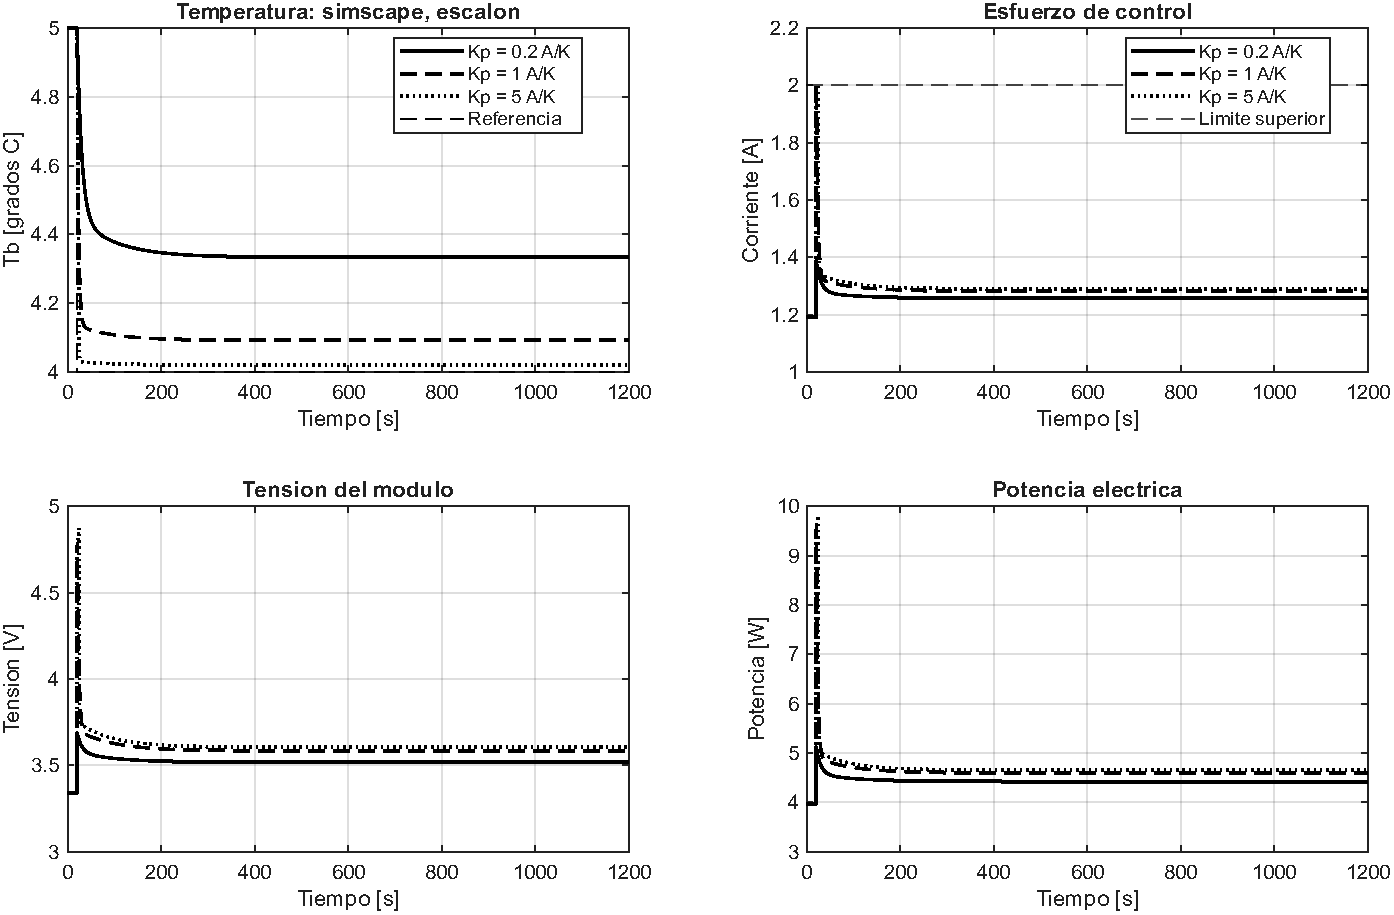
\includegraphics[width=\columnwidth]{../resultados_matlab/simscape_escalon.pdf}
\caption{Ensayo P de escalón, generado por la ejecución del modelo físico. Interpretar junto con \texttt{metricas\_P.csv}. Fuente: elaboración propia con MATLAB R2025a.}
\end{figure}
}{\pendiente{ejecutar los modelos nuevos en R2025a, verificar sus señales e incorporar las figuras y métricas realmente obtenidas.}}

La comparación definitiva debe incluir curvas de temperatura y corriente, las métricas y una interpretación por ensayo. El funcionamiento de los scripts y modelos nuevos no se certifica mediante la comprobación auxiliar.
